\chapter{Introduction}

\section{Overview}
\label{Intro: Overiew}

\section{Research context}
\label{Intro: ResearchContext}

\section{Research aim and questions}
\label{Intro:RQ}
The research described in this thesis explores the following research aim:
\begin{quote}
    \textit{``How might participation be configured for people with dementia to shape the design process of technology''}
\end{quote}
This research aim is split into three research questions, to provide insights into the experiences and perspectives of stakeholders commonly implicated in design processes in designing with and for people with dementia, intending to broaden the conversation surrounding technology design with and for people with dementia. The following section introduces each research question followed by a description.

\subsection{Research question one}
\label{RQ1}
\begin{quote}
\textit{``How can we use participatory design approaches to provide meaningful and engaging experiences for people with dementia?''}
\end{quote}
In exploring this question, the methodologies used in this thesis explore the ways to move toward more inclusive design approaches that require flexible configuration to support the different needs of participants. Further, this exploration draws attention to how we talk about dementia, to what extent people with dementia want to contribute to technology design, and ways to ensure the person with dementia is respected and engaged in research.

\subsection{Research question two}
\label{RQ2}
\begin{quote}
\textit{``What are the ethical implications for people with dementia to participate in HCI research?''}
\end{quote}
Given that people with dementia may experience changes to their ability to problem solve, increasing need for care, and make judgements, many of the social and cognitive consequences of living with dementia can be seen as ethical challenges, making it a complex space for research. With this in mind, the thesis examines ethical practices used in dementia-HCI research to present insights into the careful ethical considerations required when working with people with dementia and their families. 

\subsection{Research question three}
\label{RQ3}
\begin{quote}
\textit{``What are the competing interests and expectations to support meaningful dialogue in dementia design research when involving multiple stakeholders - such as people with dementia, developers, designers and researchers?''}
\end{quote}
For the final research question, the thesis investigates the importance of designing for multiple interests and workflows to ensure that stakeholders who are part of the design process to support collaboration and engagement between the diverse stakeholders. 

\section{Thesis structure}
\label{Intro: Thesis structure}
In this section, I describe the structure of the thesis:

\subsection{Chapter two - Background Literature}
\label{Intro:ChapterTwo}
This chapter aims to describe prior work discussing how people with dementia have been represented and involved in technology design and development. Initially, this chapter reviews the involvement of people with dementia in dementia-HCI work that draws attention to a strong relational basis for design practice. Following the review of dementia-HCI work, I highlight three areas that require investigation. From here, I draw from outside the HCI literature that examines the type of ethical dilemmas; public perception of dementia, and involving later stages of dementia in the co-creation process. Finally, to conclude this chapter, I describe four areas of interest to this thesis that might broaden our understanding of how to design and develop technology for and with people with dementia.

\subsection{Chapter three - Methodology}
\label{Intro:ChapterThree}

\subsection{Chapter four - Sharing a Virtual World with People with Dementia: A Reflective Account}
\label{Intro:ChapterFour}

\subsection{Chapter five - DemVR: Exploring Shifting Sensitivities in a Hackathon for Dementia}
\label{Intro:ChapterFive}

\subsection{Chapter six - Learning from Ethics in Dementia Research}
\label{Intro:ChapterSix}

\subsection{Chapter seven - Co-creating a Digital Toolkit to Support Design for Dementia}
\label{Intro:ChapterSeven}

\subsection{Chapter eight - Discussion and Future Work}
\label{Intro:ChapterEight}


\subsection{Thesis map}
For chapters four to seven, I present a map of which represents the different research questions each data chapter tackles (see figure \ref{fig:RQ_and_Chapters}).

\label{Intro:Thesis Map}
\begin{figure}[htp]
\centering
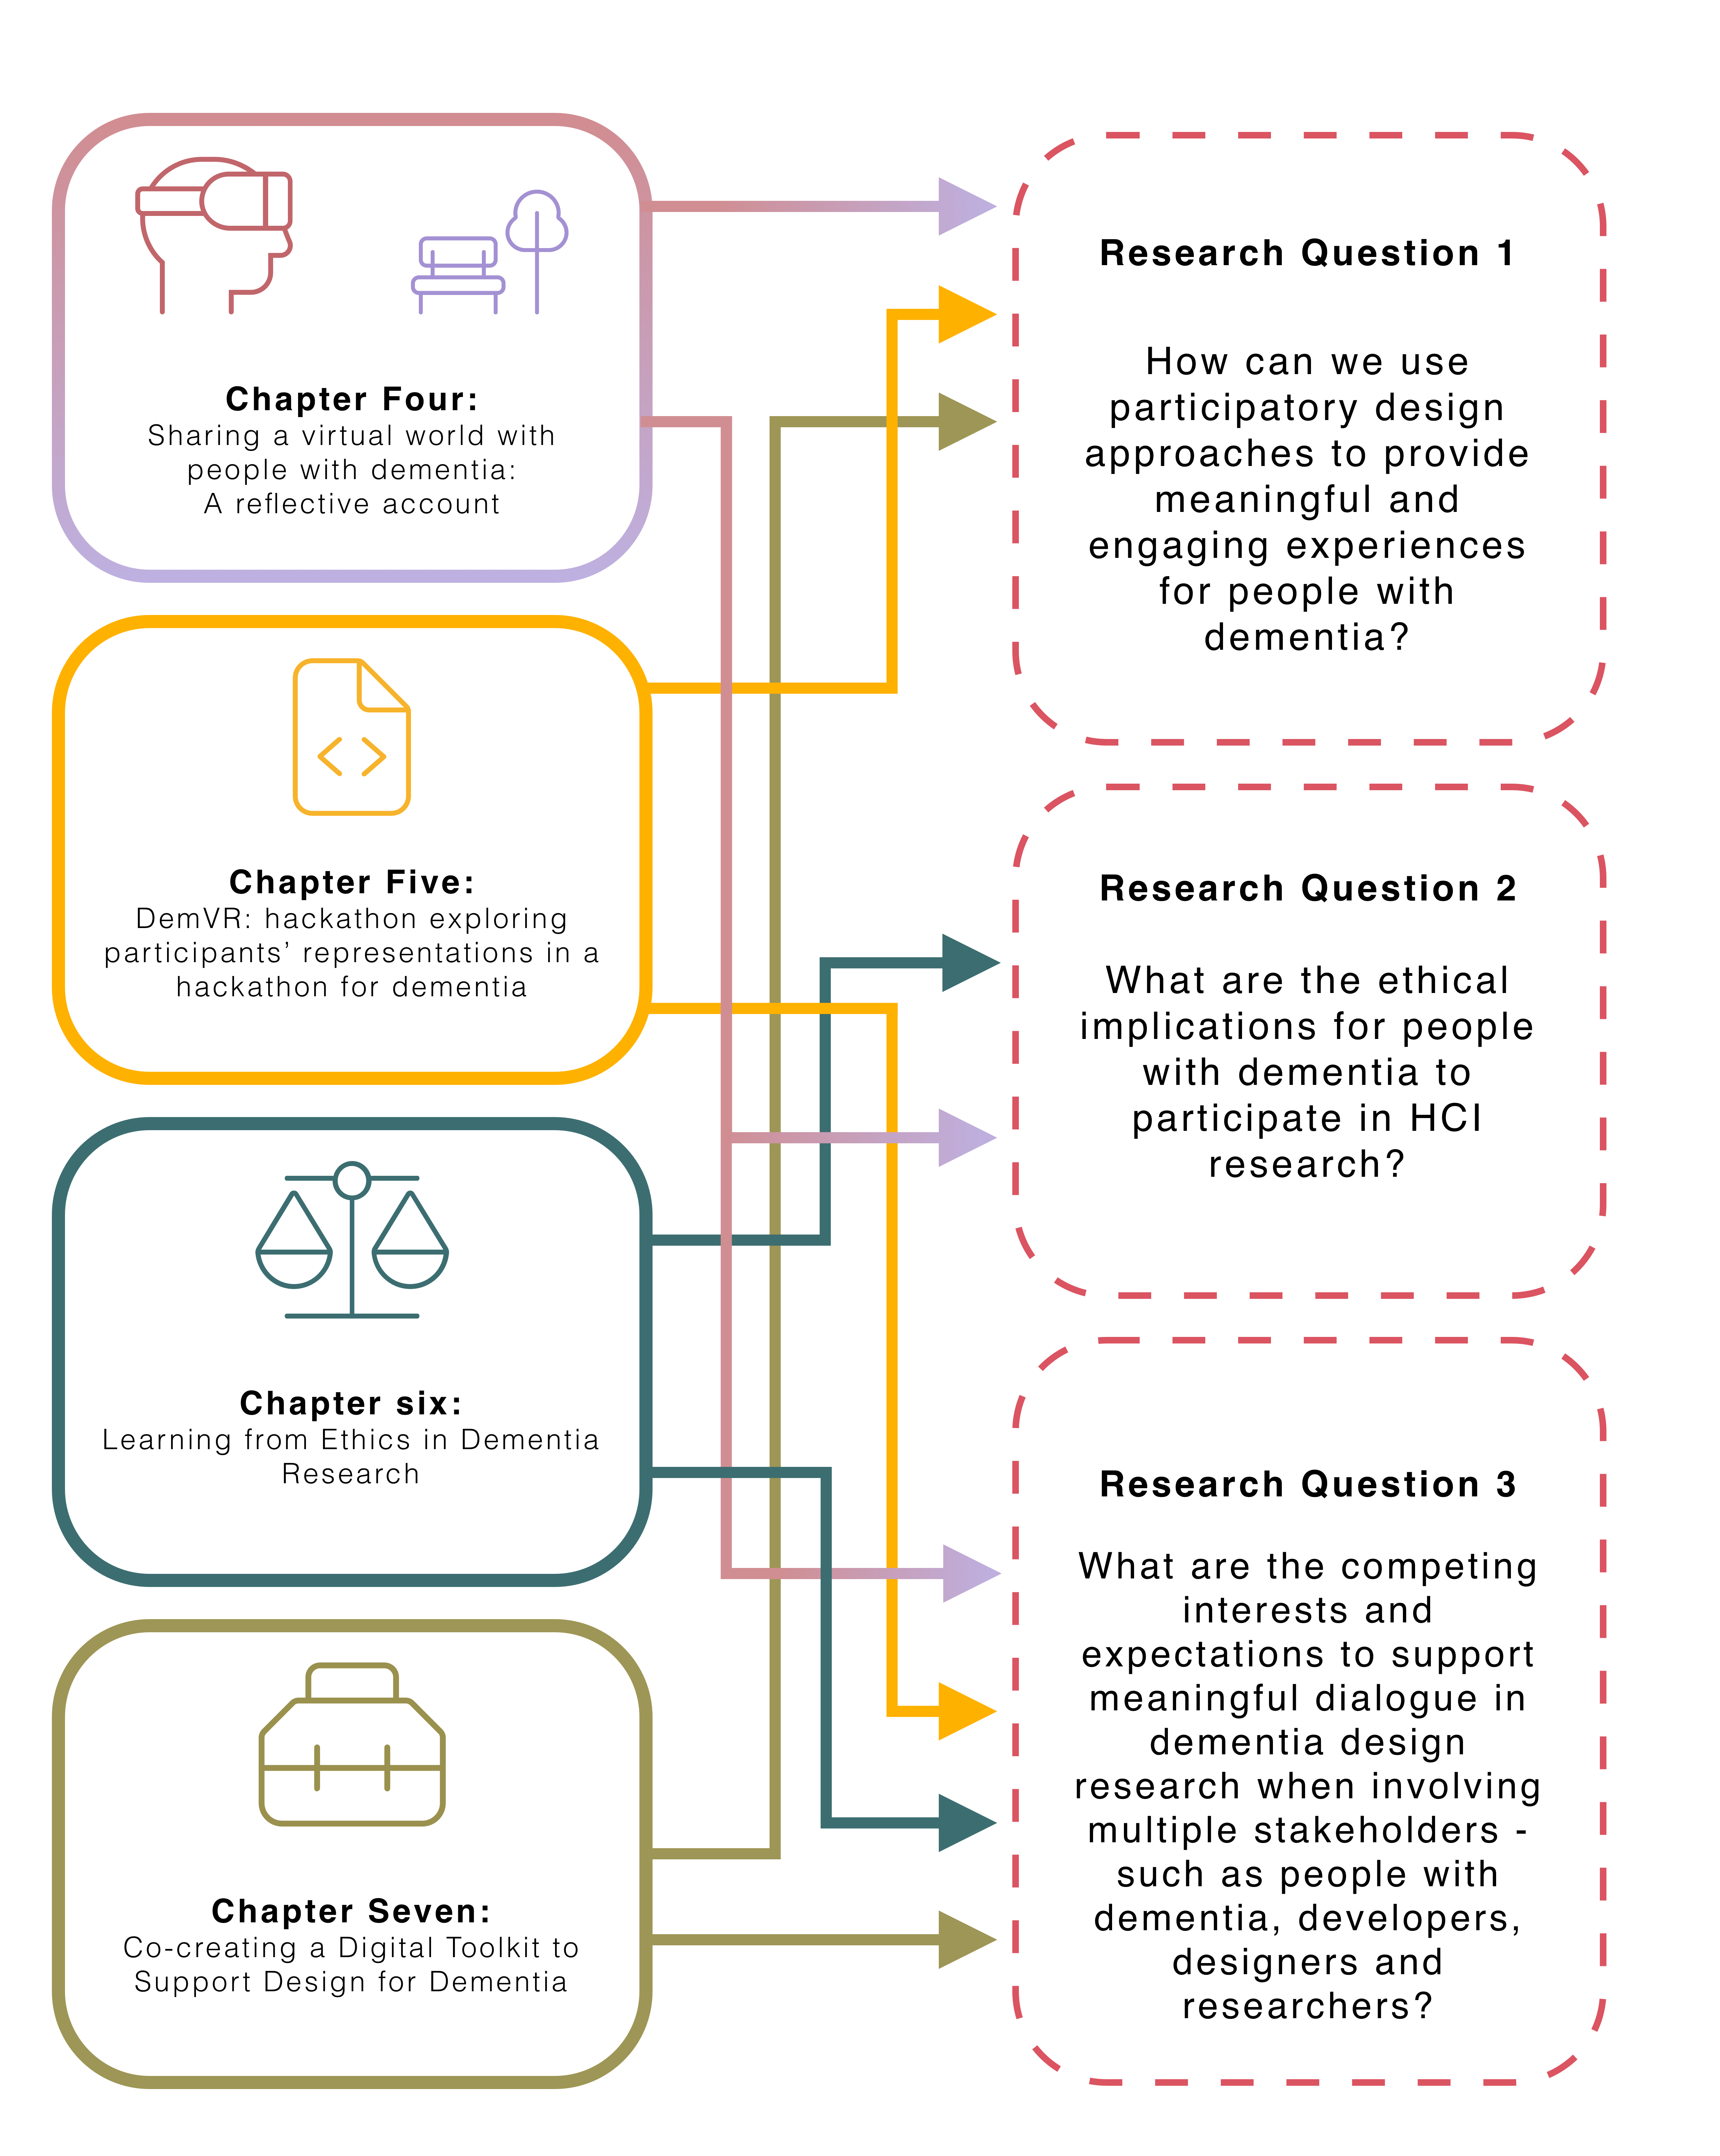
\includegraphics[width=.8\linewidth]{Images/Thesis_Narrative/RQ_and_Chapters.png}
\caption{Thesis Map showing the relationships between data chapters to research questions}
\label{fig:RQ_and_Chapters}
\end{figure}


\section{Contributions}
\label{Intro:Contribution}

\section{Summary}
\label{Intro: Summary}